%\title{Karl's Grid} 
\documentclass{article} % say
\usepackage{tikz}
\usetikzlibrary{intersections}
\tikzset{Karl's grid/.style={help lines,color=red!50,step=.5cm,very thin}}
\begin{document}
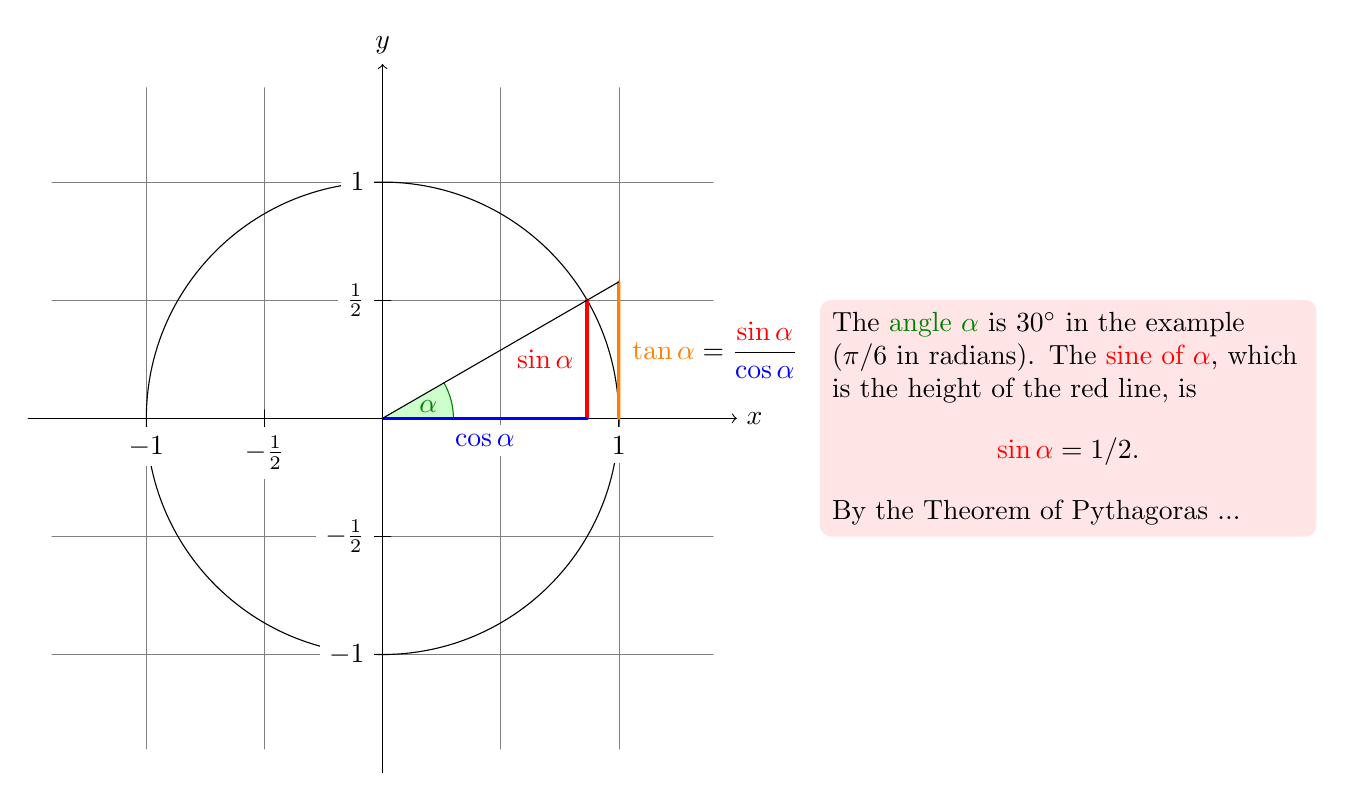
\begin{tikzpicture}
[scale=3,line cap=round,
% Styles
axes/.style=,
important line/.style={very thick},
information text/.style={rounded corners,fill=red!10,inner sep=1ex}]
% Local definitions
\def\costhirty{0.8660256}
% Colors
\colorlet{anglecolor}{green!50!black}
\colorlet{sincolor}{red}
\colorlet{tancolor}{orange!80!black}
\colorlet{coscolor}{blue}

% The graphic
\draw[help lines,step=0.5cm] (-1.4,-1.4) grid (1.4,1.4);
\draw (0,0) circle (1cm);
\begin{scope}[axes]
\draw[->] (-1.5,0) -- (1.5,0) node[right] {$x$} coordinate(x axis);
\draw[->] (0,-1.5) -- (0,1.5) node[above] {$y$} coordinate(y axis);
\foreach \x/\xtext in {-1, -.5/-\frac{1}{2}, 1}
\draw[xshift=\x cm] (0pt,1pt) -- (0pt,-1pt) node[below,fill=white] {$\xtext$};
\foreach \y/\ytext in {-1, -.5/-\frac{1}{2}, .5/\frac{1}{2}, 1}
\draw[yshift=\y cm] (1pt,0pt) -- (-1pt,0pt) node[left,fill=white] {$\ytext$};
\end{scope}
\filldraw[fill=green!20,draw=anglecolor] (0,0) -- (3mm,0pt) arc(0:30:3mm);
\draw (15:2mm) node[anglecolor] {$\alpha$};
\draw[important line,sincolor]
(30:1cm) -- node[left=1pt,fill=white] {$\sin \alpha$} (30:1cm |- x axis);
\draw[important line,coscolor]
(30:1cm |- x axis) -- node[below=2pt,fill=white] {$\cos \alpha$} (0,0);
\path [name path=upward line] (1,0) -- (1,1);
\path [name path=sloped line] (0,0) -- (30:1.5cm);
\draw [name intersections={of=upward line and sloped line, by=t}]
[very thick,orange] (1,0) -- node [right=1pt,fill=white]
{$\displaystyle \tan \alpha \color{black}=
\frac{{\color{red}\sin \alpha}}{\color{blue}\cos \alpha}$} (t);
\draw (0,0) -- (t);
\draw[xshift=1.85cm]
node[right,text width=6cm,information text]
{
The {\color{anglecolor} angle $\alpha$} is $30^\circ$ in the
example ($\pi/6$ in radians). The {\color{sincolor}sine of
$\alpha$}, which is the height of the red line, is
\[
{\color{sincolor} \sin \alpha} = 1/2.
\]
By the Theorem of Pythagoras ...
};
\end{tikzpicture}
\end{document}
